\documentclass[conference,beamer]{IEEEtran}
%usepackage[times,twocolumn,graphicx,amsmath,float,subfig,epstopdf,conference,10pt]{IEEEtran} % LaTeX 2.09
\usepackage{times}
%\usepackage{arial}
%\usepackage{twocolumn}
\usepackage{graphicx}
\usepackage{listings}
\lstset{
  basicstyle=\small\ttfamily,
 % frame=lrtb,
  %numbers=left
}
\usepackage{commath}
\usepackage{ifpdf}
\usepackage{amsmath}
\usepackage[bookmarks=false]{hyperref}
\usepackage{kantlipsum}  
%\usepackage{float}
\usepackage{dblfloatfix}  
%\usepackage{subfig}
\usepackage{subcaption}
\usepackage{epstopdf}
\usepackage{hhline}
\usepackage[table]{xcolor}
\usepackage{booktabs}
\usepackage{hyperref}
\usepackage[T1]{fontenc} % Use 8-bit encoding that has 256 glyphs
\usepackage{fourier} % Use the Adobe Utopia font for the document - comment this line to return to the LaTeX default
\usepackage[english]{babel} % English language/hyphenation
\usepackage{amsmath,amsfonts,amsthm} % Math packages
\usepackage{graphicx}
\usepackage{lipsum} % Used for inserting dummy 'Lorem ipsum' text into the template
\usepackage{cite}
\usepackage{multirow}
\usepackage{tabularray}
\usepackage{setspace}
\usepackage[rawfloats=true]{floatrow} 
\usepackage{calrsfs}
\DeclareMathAlphabet{\pazocal}{OMS}{zplm}{m}{n}
\newcommand{\RRa}{\pazocal{R}}
\newcommand{\VVa}{\pazocal{V}}
\newcommand{\AAa}{\pazocal{A}}
\newcommand{\MMa}{\pazocal{M}}
\newcommand{\SSa}{\pazocal{S}}

%\usepackage{sectsty} % Allows customizing section commands
%\allsectionsfont{\centering \normalfont\scshape} % Make all sections centered, the default font and small caps
\hypersetup{
colorlinks = true, linkcolor = blue, anchorcolor = red, citecolor = blue, filecolor = red, pagecolor = red, urlcolor = blue,
    %bookmarks=false,         % show bookmarks bar?
    unicode=false,          % non-Latin characters in Acrobat’s bookmarks
    pdftoolbar=true,        % show Acrobat’s toolbar?
    pdfmenubar=true,        % show Acrobat’s menu?
    pdffitwindow=false,     % window fit to page when opened
    pdfstartview={FitH},    % fits the width of the page to the window
    pdftitle={Simo2FC},     % title
    pdfauthor={Author},     % author
    pdfsubject={Subject},   % subject of the document
    pdfcreator={Creator},   % creator of the document
    pdfproducer={Producer}, % producer of the document
    pdfkeywords={keyword1} {key2} {key3}, % list of keywords
    pdfnewwindow=false,      % links in new window
    colorlinks=true,       % false: boxed links; true: colored links
    linkcolor=cyan,          % color of internal links (change box color with linkbordercolor)
    %citecolor=red,        % color of links to bibliography
    %filecolor=magenta,      % color of file links
    %urlcolor=cyan           % color of external linksf
  %  mathscape=true
}
\def\figureautorefname{Fig.}
\def\sectionautorefname{Section}

\usepackage{tikz}
\usetikzlibrary{shapes.geometric}

\newcommand\score[2]{
\pgfmathsetmacro\pgfxa{#1+1}
\tikzstyle{scorestars}=[star, star points=5, star point ratio=2.25, draw,inner sep=1.3pt,anchor=outer point 3]
  \begin{tikzpicture}[baseline]
    \foreach \i in {1,...,#2} {
    \pgfmathparse{(\i<=#1?"black":"white")}
    \edef\starcolor{\pgfmathresult}
    \draw (\i*1.75ex,0) node[name=star\i,scorestars,fill=\starcolor]  {};
   }
  \end{tikzpicture}
}
\usepackage{tabularx}
\usepackage{multirow}
\usepackage{fancyhdr}
\usepackage{cite}
\usepackage{balance}
\usepackage{amsmath}

\usepackage{algpseudocode}
\usepackage{algorithm}
\newcommand{\algorithmautorefname}{Algorithm}
\algnewcommand\algorithmicforeach{\textbf{for each}}
\algdef{S}[FOR]{ForEach}[1]{\algorithmicforeach\ #1\ \algorithmicdo}
\begin{document}

\title{Advanced Simulink-Based Buck Converter Modeling for Fuzzy MPPT in PV Battery Chargers}

\author{\IEEEauthorblockN{Hale Yilmaz\IEEEauthorrefmark{1}, Kemal Ozanoglu\IEEEauthorrefmark{2}, Pier Cavallini\IEEEauthorrefmark{3}, and Metin Yazgi\IEEEauthorrefmark{4}}
\IEEEauthorblockA{\IEEEauthorrefmark{1}\small{Renesas Electronics, Istanbul, TR}}
\IEEEauthorblockA{\IEEEauthorrefmark{2}\small{Department of Electrical and Electronics Engineering, Bogazici University}}
\IEEEauthorblockA{\IEEEauthorrefmark{3}\small{Cirrus Logic, Edinburgh, UK}}
\IEEEauthorblockA{\IEEEauthorrefmark{4}\small{Department of Electronics and Communications Engineering, Istanbul Technical University}}
}
\IEEEoverridecommandlockouts
\maketitle
\IEEEpubidadjcol

\begin{abstract}
Maximum Power Point Tracking (MPPT) is a crucial technique for optimizing the energy harvesting efficiency of photovoltaic (PV) battery chargers. In this work, we present an improved MPPT approach utilizing Fuzzy Logic, implemented and analyzed through Simulink simulations. While Fuzzy Logic-based MPPT methods have been widely explored, our contribution lies in the enhancement of the power conversion stage, particularly through an advanced buck converter model. Unlike conventional Simulink implementations that often rely on idealized switch models, our proposed setup incorporates a more detailed and realistic representation of buck converter switching dynamics. This refined model enables a more accurate assessment of power efficiency, transient response, and overall system performance. Simulation results demonstrate the benefits of our improved modeling approach, showcasing better prediction of losses, switching behavior, and dynamic performance under varying solar irradiation and load conditions. These findings contribute to the design of more efficient and reliable PV battery chargers for renewable energy applications.  
\end{abstract}

% SIBO ? / title ?
% Hale will update Figs 4 & 5
% Fig 4: labels illegible, yellow illegible DVL is not needed
% DFC instead use DVCF1

\begin{IEEEkeywords}
DC-DC converters, SIDO converter, hybrid converter, power management integrated circuits, flying capacitor, AMOLED display.
\end{IEEEkeywords}

\section{Introduction}
Together with the increasing demand for portable applications, display drivers necessitating large positive and negative power supply voltages have become popular, such as active-matrix organic light-emitting diode (AMOLED) and passive-matrix organic light-emitting diode (PMOLED) drivers. The positive and negative power supply voltages are typically provided by two independently regulated DC-DC converters, a boost converter, and an inverting buck-boost converter, respectively. However, the mentioned configuration requires two inductors, leading to an increase in the development cost and an increase in the board area. Single-inductor dual-output (SIDO) structures with bipolar output voltage rails (generating both positive and negative supply) are preferred in portable applications, as a single inductor offers reduced EMI (Electromagnetic Interference) and board area. Examples are reported in \cite{simo3,simo4}, and in products like TPS65135 \cite{TPS65135}.

\begin{figure}[ht]
\centerline{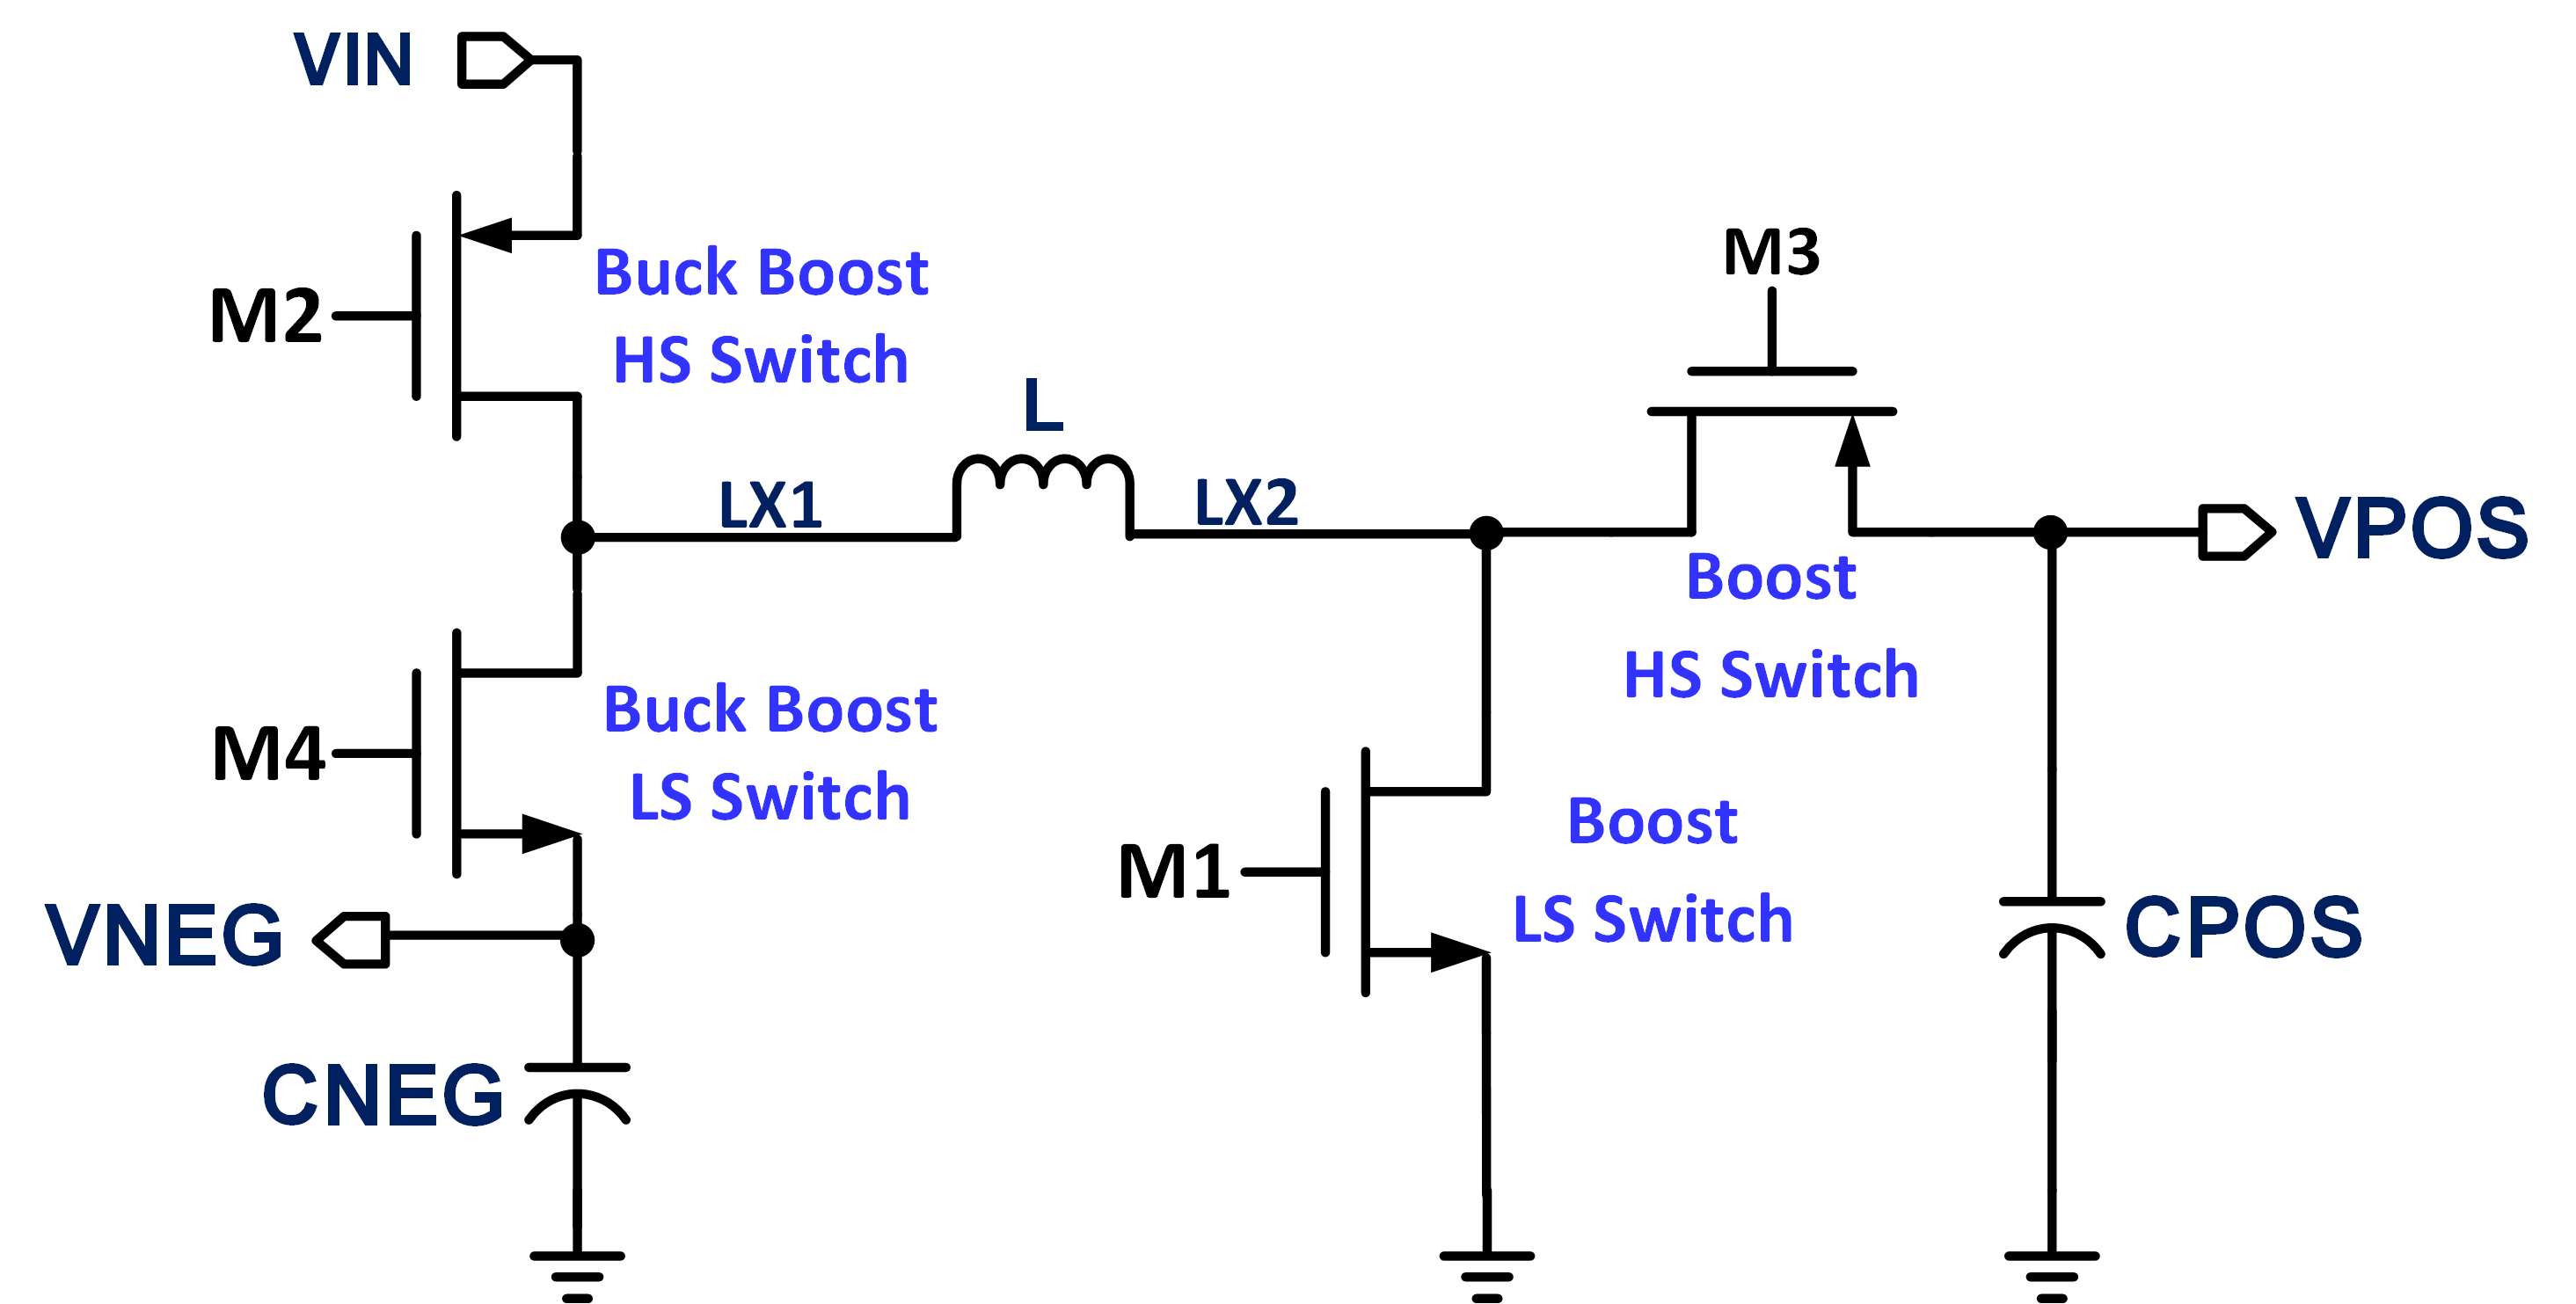
\includegraphics[width=0.85\columnwidth]{simo_conventional.png}}
\caption{Conventional SIDO converter.}\label{conventional_simo}
\end{figure}

A conventional single-inductor multiple-output (SIDO) regulator topology with positive and negative output voltage rails is given by \autoref{conventional_simo}. To generate the negative output voltage $V_{NEG}$, the switching sequence of the regulator is as follows: in the first phase, when magnetizing the inductor, $M_1$ and $M_2$ are $ON$, the inductor current is increasing with a slope of $V_{IN}/L$, where $V_{IN}$ is the input supply voltage. In the second phase, when de-magnetizing the inductor, $M_1$ and $M_4$ are $ON$, the inductor current is decreasing with a slope of -$V_{NEG}/L$. Current in the inductor is flowing to the ground through $M_1$ while reducing the voltage on $C_{NEG}$ through $M_{4}$, thus generating a negative voltage at the output $V_{\mathit{NEG}}$.  According to inductor volt-second balance and  power balance equations, the converter voltage conversion ratio and average inductor current can be derived as in \autoref{eq_vc_nfc}.

\begin{equation}
\frac{Vout}{Vin}=\frac{D}{1-D} \qquad I_{\mathit{L(avg)}}=\frac{1}{1-D}I_{\mathit{out}}
\label{eq_vc_nfc}
\end{equation}

There exist various topology limitations of this converter regarding negative output voltage generation: during de-magnetization phase, the inductor observes a voltage drop close to $V_{\mathit{NEG}}$. For significantly low values of $V_{\mathit{NEG}}$ (e.g., $-20V$ for an AMOLED application), this voltage drop will result in high inductor current ripple and core losses \cite{powerbook}, leading to a decrease in power efficiency. Higher ${\partial I_L}/{\partial t}$ during this phase also results in increased reverse recovery loss for MOSFET switches. In addition to that, during the magnetization phase of the inductor, $M_{4}$ observes a $V_{DS}$ of $|V_{\mathit{NEG}}|+V_{IN}$, which sets a relatively high voltage constraint on the switch device safe operating region. 

\begin{figure}[ht]
\centerline{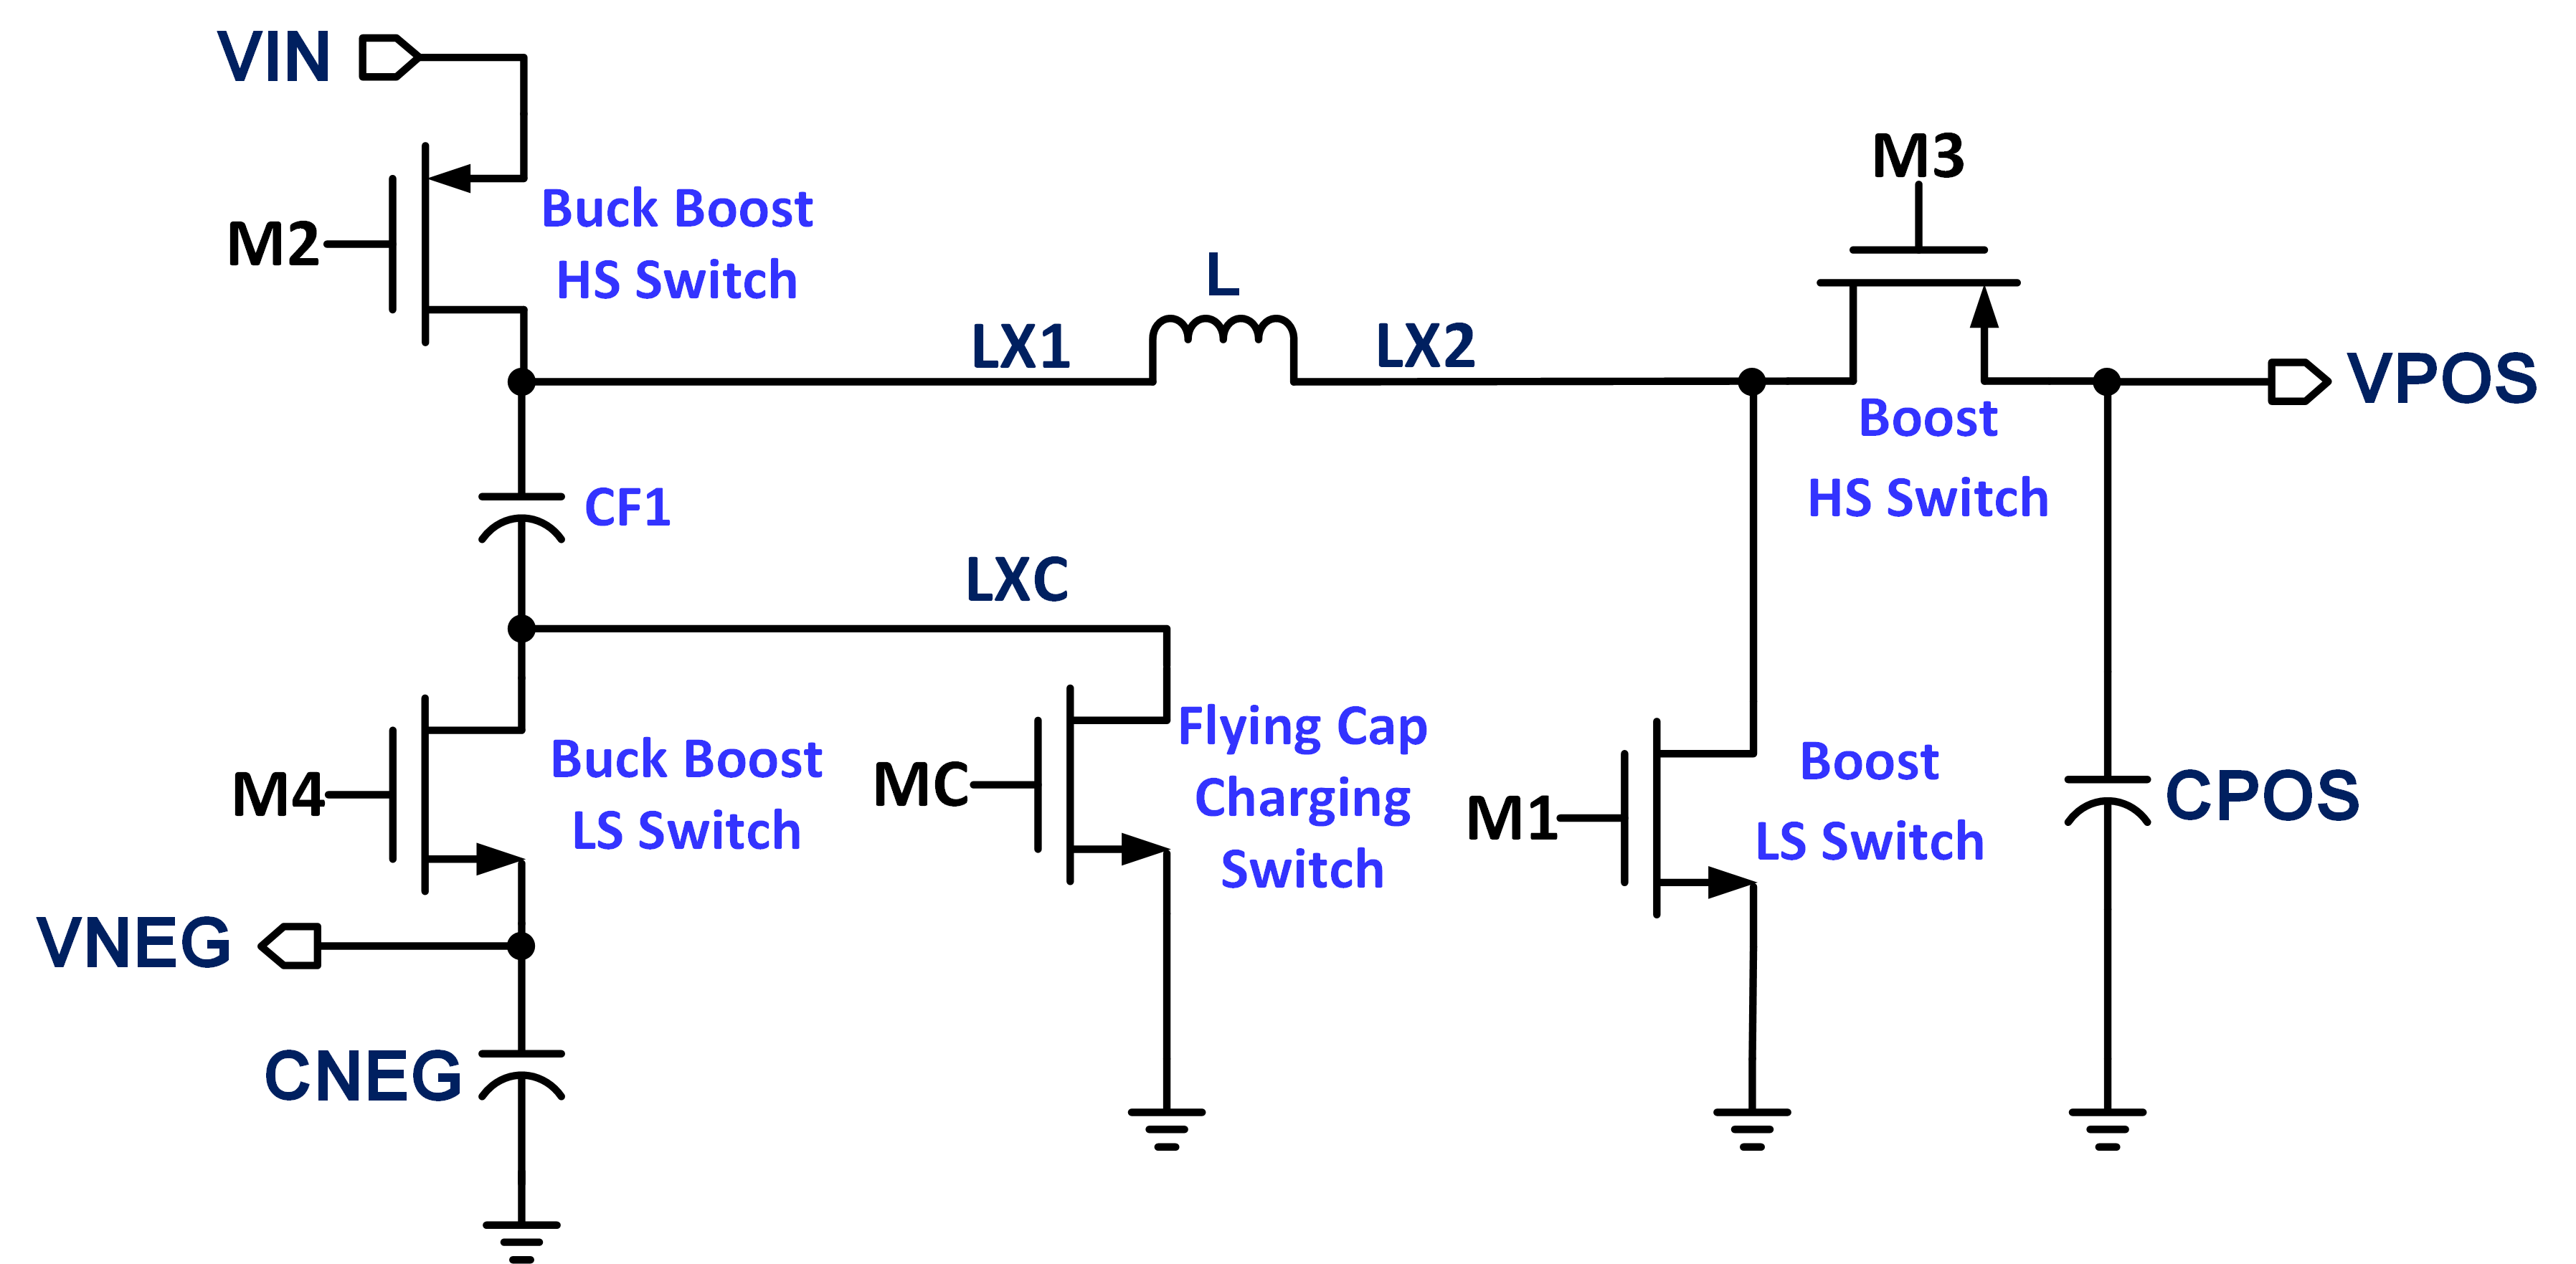
\includegraphics[width=0.9\columnwidth]{simo_1fcap.png}}
\caption{SIDO with one Flying Capacitor} \label{simo_1fc}
\end{figure}

Hybrid topologies utilizing flying capacitors are proposed, aiming to reduce voltage stress on active switching components, hence allowing design with less resilient devices that are more efficient in terms of silicon area. By further reducing the voltage drop over the coil during the de-magnetization phase, the flying capacitor also helps decrease the inductor current ripple, the average inductor current, and the maximum inductor current. Consequently, lower core losses and AC losses can be obtained. These advantages lead to the flexibility of using smaller coils. Decreasing the maximum inductor current also enables converter operation at higher ambient temperatures due to lower losses. This will prevent saturation of the core and possible damage to the regulator.
Another advantage of hybrid topologies is that they enable the switching converter to operate with lower duty cycle for the given load current, which relaxes the system stability requirements considering sub-harmonic oscillation and the output voltage collapse issue \cite{boostcollapse}. Reduction in the inductor current ripple will also alleviate the EMI noise generated by the converter.
The trade-off of adding the flying capacitor is increasing in switching and resistive losses introduced by the additional switches to the topology.

% optional references {sibo1,sibo2,sibo3,sibo4,sibo5}
To address the mentioned performance improvements, a SIDO converter with a flying capacitor has been presented in the literature, such as \cite{sibo2,sibo3,sibo5}.
\autoref{simo_1fc} shows the topology of a SIDO converter with one flying capacitor (1FC). The operating principle is described as follows: in the first phase, when magnetizing the inductor, $M_{1}$, $M_{2}$, and $M_{C}$ are $ON$. The inductor current is increasing with a slope of $V_{IN}/L$ and $C_F$ is charged to $V_{IN}$ through the input supply and $M_C$. During this phase, the $V_{DS}$ voltage drop on $M_{4}$ is reduced to $|V_{\mathit{NEG}}|$-$V_{IN}$, which relaxes the voltage constraint on the switch by a $V_{IN}$, with respect to the conventional SIDO converter given by \autoref{conventional_simo}. In the second phase, when de-magnetizing the inductor, $M_{1}$ and $M_{4}$ are $ON$. Voltage drop on the inductor is reduced to $|-V_{NEG}+V_{IN}|$, thus the ${\partial I_L}/{\partial t}$ slope is decreased. According to the inductor-volt second balance and  power balance equations, the voltage conversion ratio and average inductor current can be obtained as given by \autoref{eq_vc_1fc}. 

\begin{equation}
\frac{Vout}{Vin}=\frac{1}{1-D}  \qquad I_{\mathit{L(avg)}}=\frac{1}{1-D}I_{\mathit{out}}
\label{eq_vc_1fc}
\end{equation}

Multiple flying capacitors can be stacked in the topology, allowing further reduction on the voltage drop over the inductor during de-magnetization phase by $n \cdot V_{IN}$, where $n$ is the number of flying capacitors. 

This paper investigates the SIDO structure using two flying capacitors (2FC), utilizing the benefits of hybrid converter topology by further relaxing coil constraints and achieving better power efficiency and lower duty cycle, both for negative and positive output voltage generation.  

The paper is organized as follows: Section II introduces the architecture of the proposed SIDO converter topology with two flying capacitors and shows operation phases for both negative voltage and positive voltage generation. Section III presents the simulation results together with an evaluative comparison with no flying capacitor (NFC), one flying capacitor (1FC), and two flying capacitors (2FC) topologies. Finally, Section IV presents the conclusions. 

\section{SIDO Converter with 2 Flying Capacitors}

\subsection{Negative Output Voltage Generation}

 To alleviate the aforementioned issues and to improve the switching converter performance, a second flying capacitor is introduced to the SIDO converter topology. The proposed SIDO converter is illustrated in \autoref{simo2sw} \cite{patent}. The second flying capacitor, $C_{F2}$ is introduced to the circuit in series with the first flying capacitor and $M_2$. $M_{C2}$ is added to the circuit to create the path from $V_{IN}$ to the ground while charging the second flying capacitor to the supply voltage $V_{IN}$ at the first phase. The bypass switch $M_{4}$ creates the path from $V_{IN}$ when charging the second flying capacitor. The coupling switch $M_2$ allows to connect two flying capacitors in series when the inductor current is discharging, therefore improving the inductor voltage drop at the de-magnetization phase by $2 \cdot V_{IN}$. 

 % optional text
 % A design option to switch between 1FC topology and 2FC topology also exists, by connecting the source terminal of $M_{4}$ to $LX1$ node, providing modularity to the topology.

\begin{figure}[!h]
\centerline{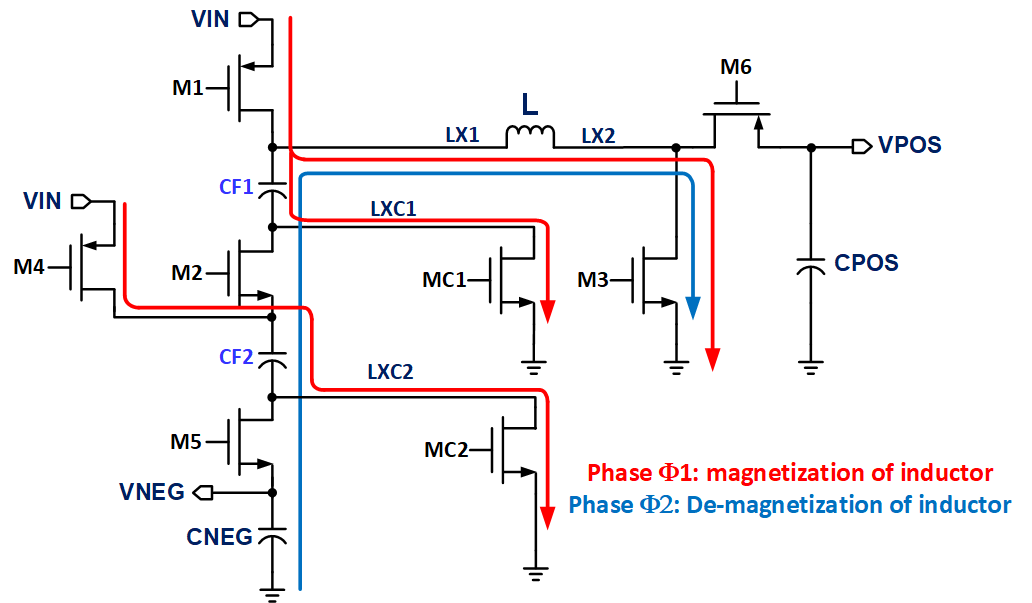
\includegraphics[width=1\columnwidth]{simo_2fcap_phases.png}}
\caption{Proposed SIDO 2FC converter and switching phases for negative voltage generation.} \label{simo2sw}
\end{figure}

To generate negative output voltage, switch states are as follows: in the first phase, when magnetizing the inductor, $M_{1}$, $M_{C1}$, $M_{C2}$, $M_{4}$, and $M_{3}$ are $ON$. The inductor current is increasing with a slope of $V_{IN}/L$. During this phase, the two flying capacitors are charged up to $V_{IN}$. When de-magnetizing the inductor, $M_{3}$, $M_{5}$, and $M_{2}$ are $ON$. The inductor current is decreasing with a slope of $|-V_{NEG} +2 V_{IN}|/L$. \autoref{simo2sw} illustrates the operation phases. According to inductor volt-second balance and power balance equations, the voltage conversion ratio and the average inductor current of the converter can be obtained by \autoref{eq_vc_2fc}.

\begin{equation}
\frac{Vout}{Vin}=\frac{(2-D)}{(1-D)} \qquad  I_{\mathit{L(avg)}}=\frac{1}{(1-D)}I_{\mathit{out}}
\label{eq_vc_2fc}
\end{equation}

 By charging up the two flying capacitors approximately to $V_{IN}$, now the inductor observes a voltage drop of $|-V_{NEG}+2\cdot V_{IN}|$; consequently, the proposed SIDO converter achieves less average inductor current with less ripple and improved core losses. \autoref{eq_vc_2fc} also shows that for the same voltage conversion ratio, the SIDO 2FC topology can operate with lower duty cycles compared to 1FC and NFC topologies.
 
\subsection{Positive Output Voltage Generation}

The mentioned improvements also apply to  positive output voltage generation using positive buck-boost switching sequence. Referring to \autoref{simo2sw}, in the first phase, when magnetizing the inductor, $M_{1}$, $M_{3}$, $M_{4}$, $M_{C1}$, and $M_{C2}$ are $ON$. The inductor current is increasing with a slope of $V_{IN}/L$. Meanwhile, the two flying capacitors are charged up to $V_{IN}$, similar to the negative voltage operation. In the second phase, when de-magnetizing the inductor, $M_{C2}$, $M_{2}$, and $M_{6}$ are $ON$. The inductor current is decreasing with slope of $|2\cdot V_{IN}-V_{POS}|/L$. Thus, by using the 2FC topology, the voltage drop on the inductor is reduced by $2\cdot V_{IN}$, with respect to the NFC topology.
The voltage conversion ratio of the 2FC topology for positive voltage operation can be found to be the same as for negative voltage operation, given by \autoref{eq_vc_2fc}.

\section{Simulation Results}

To evaluate the mentioned topologies, the NFC, 1FC and 2FC designs are modeled and simulated in Cadence Virtuoso Analog Design Environment. The switch elements are modeled with $50m\Omega$ $(M_2, M_3, M_4, M_6)$ and $30m\Omega$ $(M_1, M_{C1}, M_{C2})$ on-resistance, with $10pF$ gate capacitance, and body diodes. Non-overlap logic is introduced during the switching sequences to prevent shoot-through.
The passive components used in the simulation setup are: $L=1\mu H$ with $R_{DCR}$=10m$\Omega$ (VCMT053T-1R0MN52M), $C_{F1}$=$C_{F2}$=1$\mu$F with $R_{ESR}$=6m$\Omega$ (GRM219B31E105KA88), $C_{out}$=30$\mu$F with $R_{ESR}$=3m$\Omega$ (GRM155R61A106ME18). 

To model the core losses, the subcircuit described in \cite{coreloss} is included in the simulation test bench. The core loss coefficients are derived from the applet provided by the manufacturer for the selected inductor\cite{calculator}.

An example of target specifications for the converter, intending to address mobile AMOLED, PMOLED and Light Sensor applications are given by \autoref{specs}. 

\autoref{simo2tran} shows the transient simulation waveform of 2FC topology for negative output voltage generation. The control method used in this work is continuous conduction mode (CCM)  with peak current control at 3MHz system clock frequency. With the rising edge of the system clock $CLK$, the first phase switch control voltage $gN$ is set to high, and the inductor current $I_L$ starts to increase. When $I_{pk}$ hits $I_{lim}$ (the inductor current sense signal), the second phase starts and the inductor current starts to decrease. $\Delta V_{CF1}$ and $\Delta V_{CF2}$ demonstrate the voltage drop on the first flying capacitor $C_{F1}$, and the second flying capacitor $C_{F2}$ which are charged to $V_{IN}$ during the first phase. $\Delta B$ shows the estimated magnetic flux density obtained with the model proposed in\cite{coreloss} to calculate core losses. $V_{NEG}$ is the output voltage settling at an average target value of -10V.

\begin{figure}[!h]
\centerline{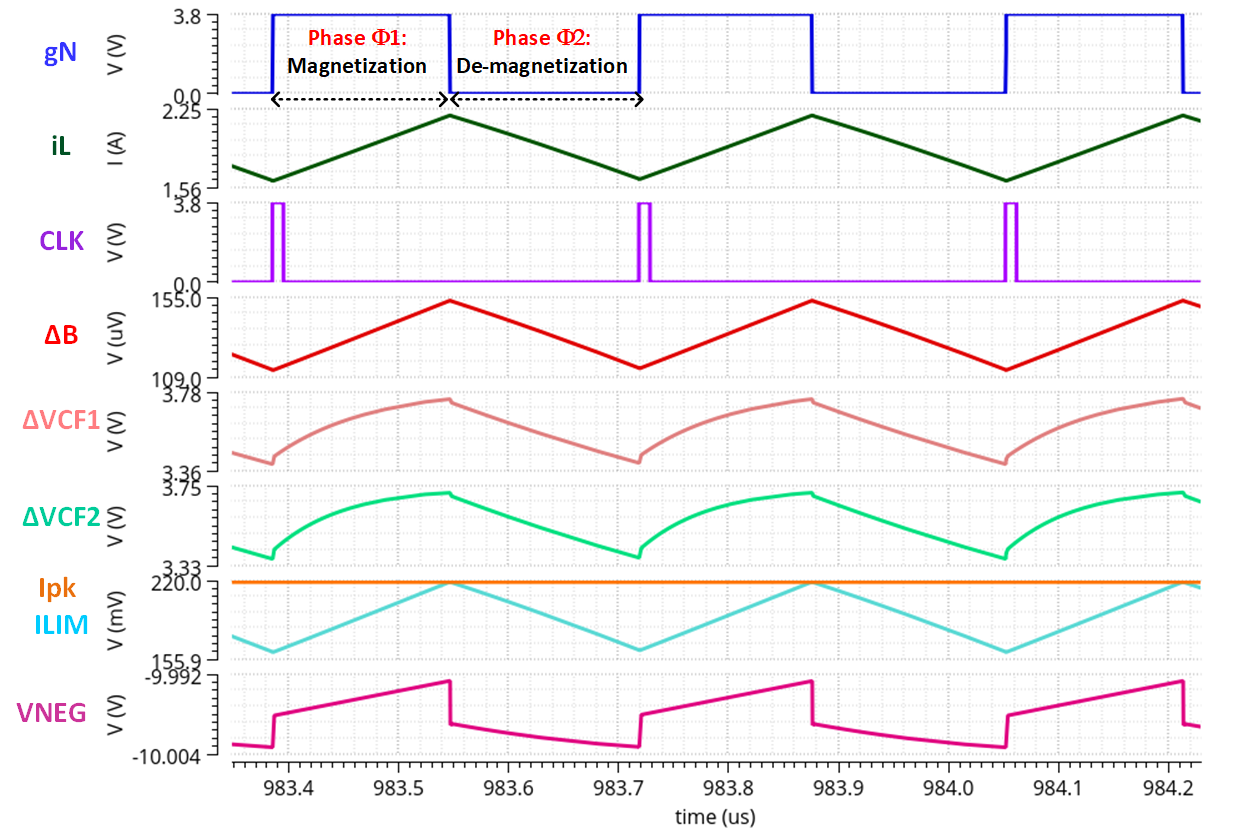
\includegraphics[width=1\columnwidth]{simo_transient4.png}}
\caption{Transient simulation results of proposed SIDO converter.} 
\label{simo2tran}
\end{figure}

\begin{table}[!h]
\centering
    \caption{System Specifications}
    \label{specs}
   \begin{tabular}{l|c|r|l}
     \textbf{Parameter} & \textbf{Value}  \\
     \hline
     $V_{IN}$ & 2.5V / 3.8V \\ % <--
     $V_{NEG}$ & -10V \\ % <--
     $V_{POS}$ & 8V \\ % <--
     $F_{CLK}$ & 3MHz  \\ % <--
     $I_{Load}$ & 1A \\ % <--
\end{tabular}

\end{table}

\autoref{tab:vneg_results} tabulates the simulation results of negative output voltage generation for the given specifications. The power efficiency results include modeled conduction losses, core losses, parasitic gate capacitance losses and body diode losses. It is observed that the power efficiency increases from NFC topology to 1FC topology and increases further with using 2FC topology. For the minimum input supply voltage condition $(V_{IN}=2.5V)$, up to 4.9\% improvement with the 1FC topology and 7.7\% improvement with the 2FC topology are observed, compared to the conventional NFC topology. The duty cycle decreases as flying capacitors are inserted into the circuit. The inductor current ripple decreases similarly as a result of decreasing voltage drop over the coil, which results in core loss reduction. The 2FC topology also achieves less inductor peak current, which helps in relaxing the magnetic core saturation constraints and alleviates possible die-heating issues. 

\begin{table}[!h]
\centering

\caption{Negative output voltage simulation results}
    \label{tab:vneg_results}
\begin{tabular}{c|c|ccc}

\multicolumn{1}{c}{} & \multicolumn{1}{c}{} & \multicolumn{3}{c}{\textbf{Topology}}  \\
\cmidrule(rl){3-5} 
\textbf{$V_{IN}$(V)} &\textbf{Parameter} & \textbf{NFC} & \textbf{1FC} & \textbf{2FC} \\
\midrule
\multirow{3}{*}{{2.5}}
 & Efficiency (\%) & 72.3 & 76.1 & 81  \\
 & Duty Cycle (\%) & 84 & 80 & 74  \\
 & Core Loss (mW) & 55 & 39 & 21 \\
 & $\Delta I_{L}$ (mA) & 0.7 & 0.66 & 0.55  \\
 & Max $I_{L}$ (A) & 6.65 & 5.54 & 4.2  \\
 \hline 
\multirow{3}{*}{{3.8}}
 & Efficiency (\%) & 85.8 & 88.7 & 90.5  \\
 & Duty Cycle (\%) & 75 & 66 & 47 \\
 & Core Loss (mW) & 65 & 45 &  27 \\
 & $\Delta I_{L}$ (mA) & 0.86 & 0.77 & 0.57  \\
 & Max $I_{L}$ (A) & 4.49 & 3.34 & 2.18  \\
\bottomrule
\end{tabular}
\end{table}

\autoref{piechart} presents the breakdown of the contributions to the power losses for the proposed topology. The major loss contributors are the introduced switches $M_{C2}$, $M_{2}$, and $M_{4}$, which contribute approximately 30\% of the total power loss.

\begin{figure}[!h]
\centerline{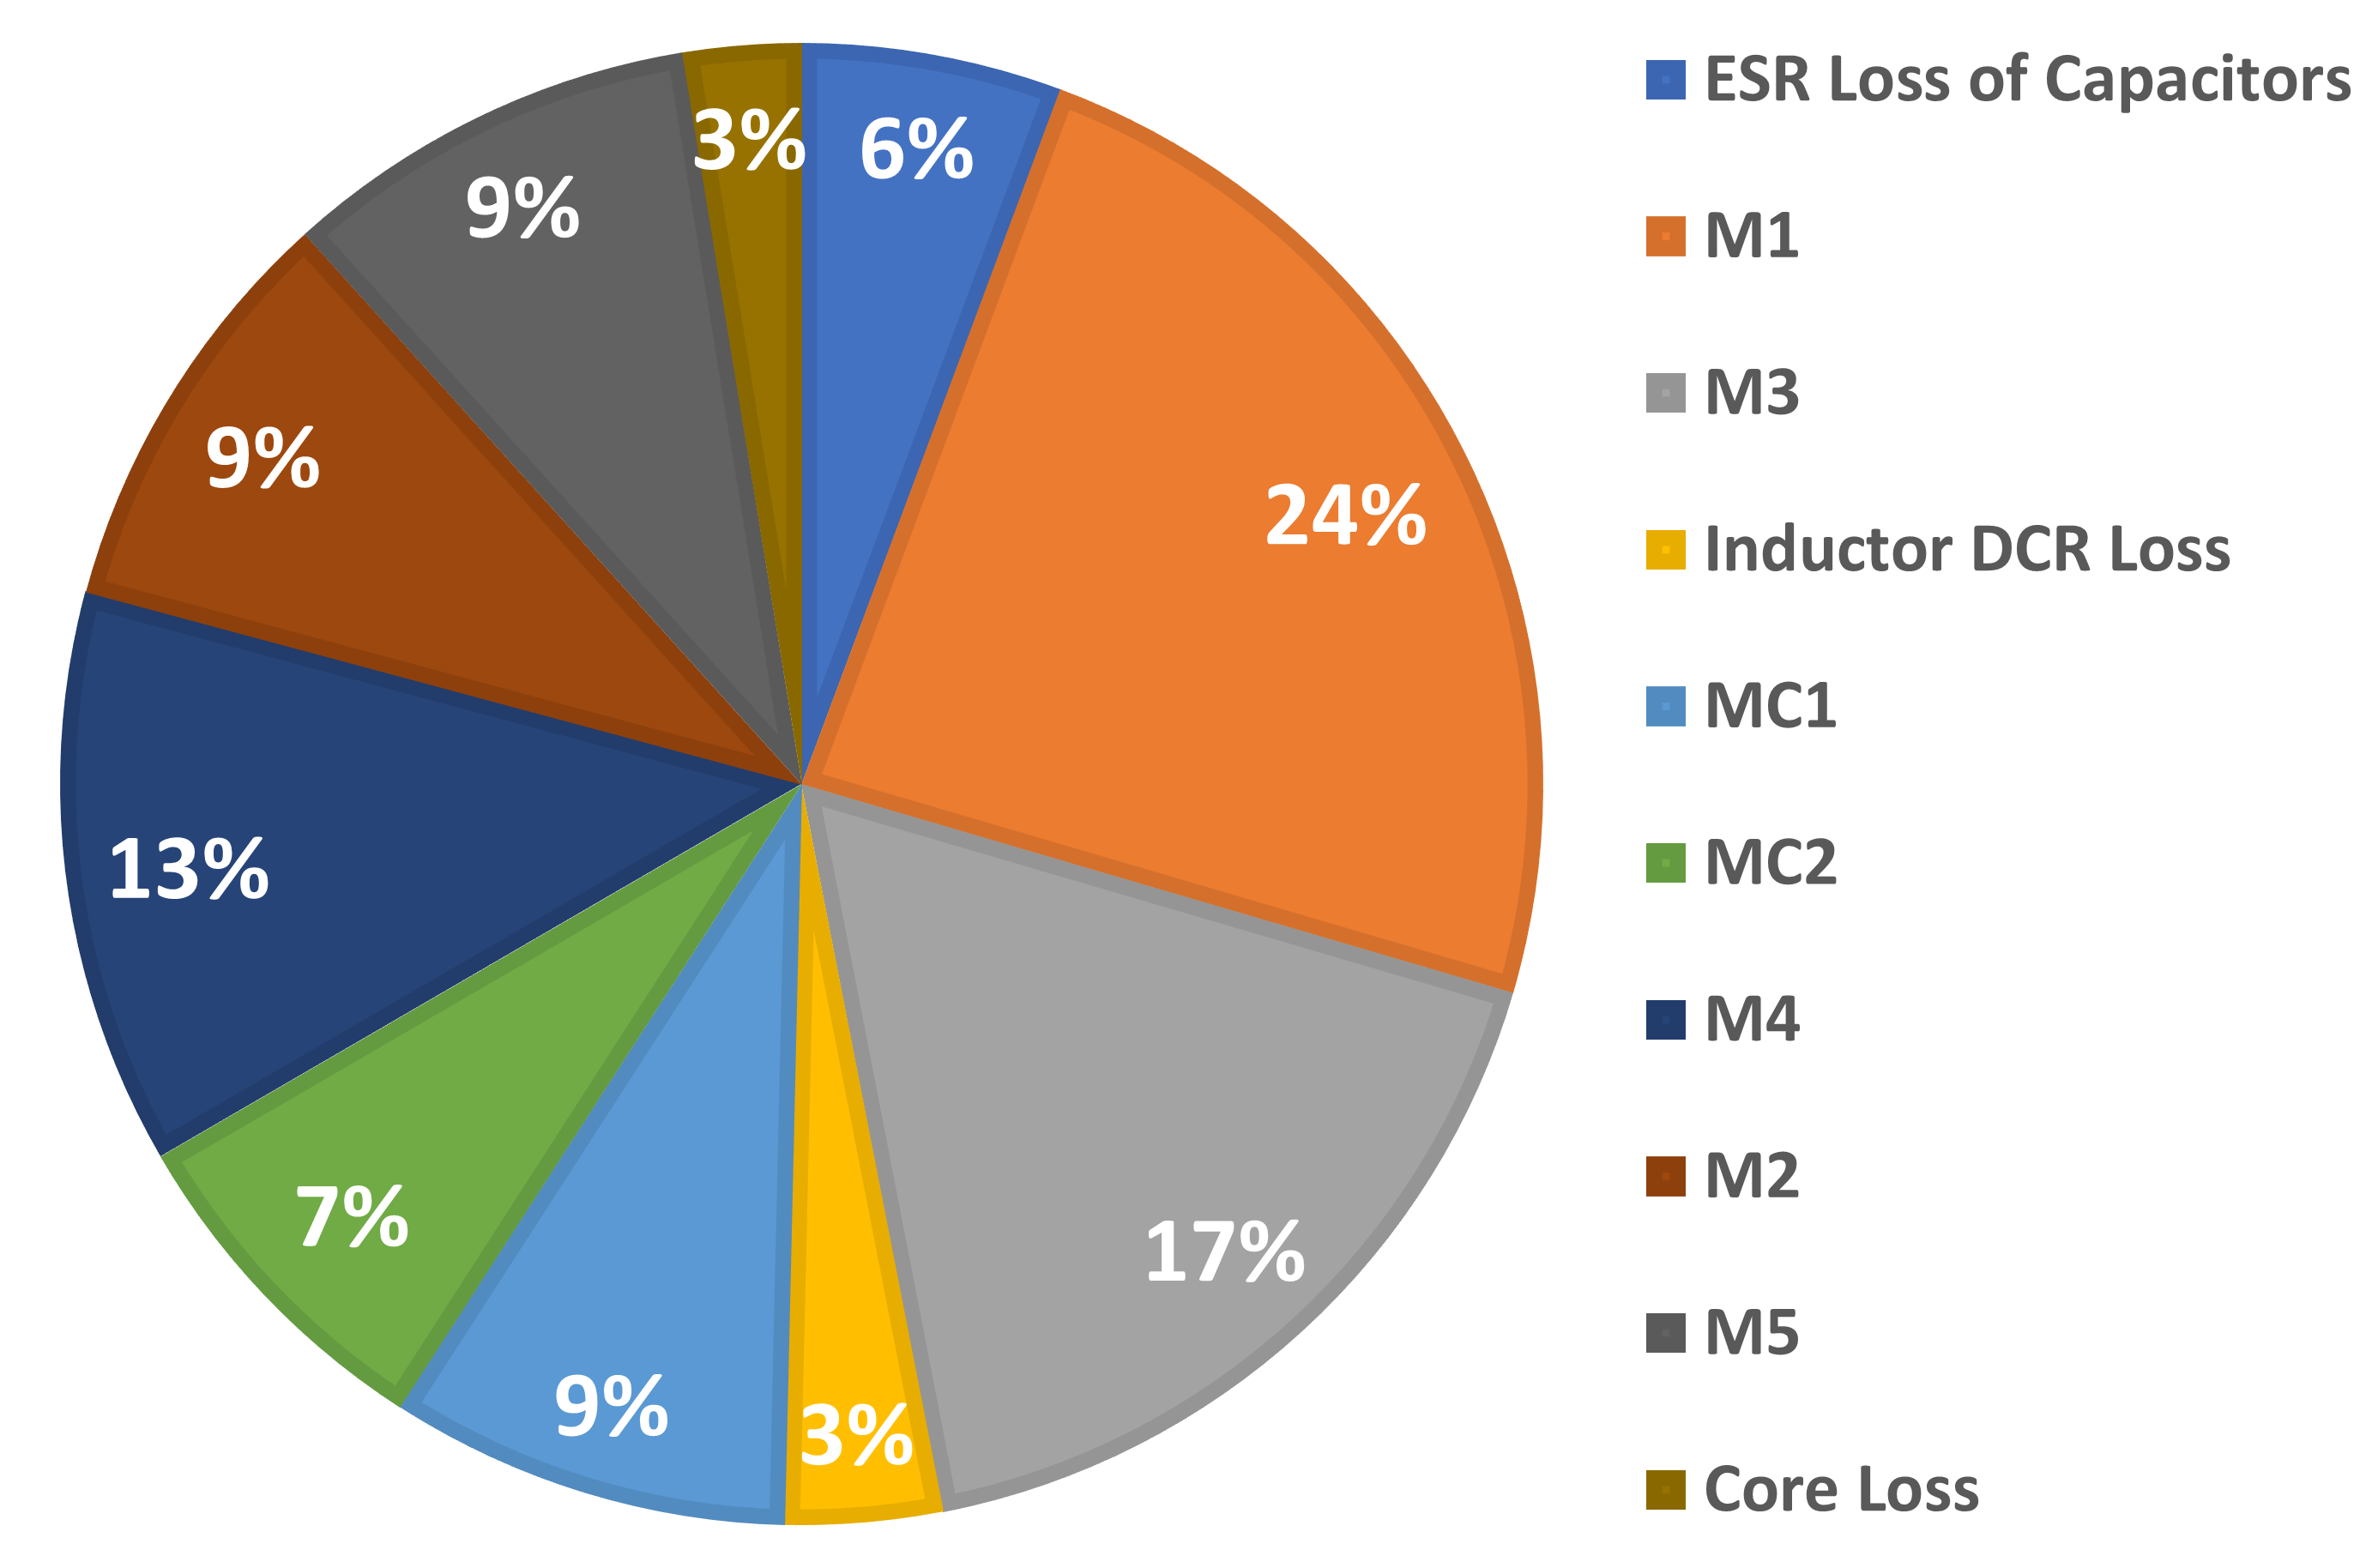
\includegraphics[width=0.8\columnwidth]{pie_chart.png}}
\caption{Simulated power loss breakdown for negative output voltage generation for $V_{IN}$=3.8V} \label{piechart}
\end{figure}

\autoref{tab:vpos_results} shows simulation results for positive output voltage generation for the specifications given by \autoref{specs}. The previously mentioned performance improvements are also observed in this configuration. Essentially, better power conversion efficiency with relaxed coil current constraints are achieved with the proposed multiple flying capacitor topology. For the $V_{IN}=3.8V$ case, even though the efficiency numbers for 1FC and 2FC topologies are observed to be similar, the 2FC topology still can be the preferred option owing to the advantage of lower duty cycle operation with relaxed coil current constraints.

\begin{table}[h]
\centering
\caption{Positive output voltage simulation results}
    \label{tab:vpos_results}
\begin{tabular}{c|c|ccc}
\multicolumn{1}{c}{} & \multicolumn{1}{c}{} & \multicolumn{3}{c}{\textbf{Topology}}  \\
\cmidrule(rl){3-5} 
\textbf{$V_{IN}$(V)} &\textbf{Parameter} & \textbf{NFC} & \textbf{1FC} & \textbf{2FC} \\
\midrule
\multirow{3}{*}{\centering{2.5}} 
 & Efficiency (\%) &74.9 & 80.8  & 83.7  \\
 & Duty Cycle (\%) & 83 & 75 & 66  \\
 & Core Loss (mW) & 120 & 91 & 63 \\
 & $\Delta I_{L}$ (A) & 1.85 & 0.99 & 0.67  \\
 & Max $I_{L}$ (A) & 5.97 & 4.3 & 3.13  \\
 \hline 
\multirow{3}{*}{{3.8}} 
 & Efficiency (\%) & 87.7 & 89.2 & 88.9  \\
 & Duty Cycle (\%) & 71 & 57 & 28   \\
 & Core Loss (mW) & 98 & 75 &  22 \\
 & $\Delta I_{L}$ (A) & 1.3 & 1.1 &  0.35 \\
 & Max $I_{L}$ (A) & 3.95 & 2.84 & 1.52  \\
\bottomrule
\end{tabular}
\end{table}

\section{Conclusion}

A novel SIDO DC-DC converter with two flying capacitors is presented. The topology aims to reduce the voltage drop on the inductor compared to the conventional converters, targeting to improve core losses and power efficiency, reduce peak inductor current and ripple while operating with lower duty cycles for both negative and positive output voltage generation. Simulation results show a reduction in inductor peak current and inductor ripple, along with low duty cycle operation, which leads to relaxed converter stability and coil current constraints. Simulations with given display driver application specifications show up to 7.7\% efficiency improvement compared to the conventional SIDO converter and up to 4.9\% efficiency improvement compared to the SIDO converter with one flying capacitor topology. Even though the technique is described through the example of a SIDO converter, the proposed technique can be applied to other hybrid switching converter topologies. 

% optional text 
% To our best knowledge, this is the first work in the literature employing multiple flying capacitors on the same voltage rail, presenting performance improvements of the hybrid topology. 



\section*{Acknowledgements}
This work was supported by Renesas Electronics, Bogazici University, and Istanbul Technical University. 

\bibliographystyle{IEEEtran}
\bibliography{IEEEabrv,ref}

\end{document}

